\subsection{23 августа.  Пер. Джалпаккол Северный (1А)}
\textit{Метеоусловия: утром: ясно, тепло, после 16:00 туман, дождь, вечером ясно.}

\begin{figure}[h!]
	\centering
	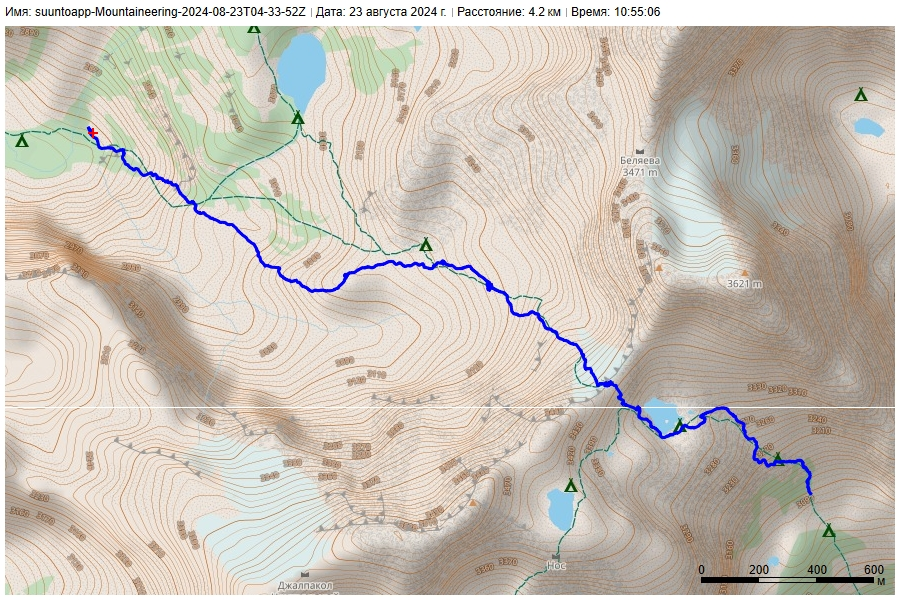
\includegraphics[angle=0, width=0.7\linewidth]{../pics/mini_maps/23}
	\label{fig:mini_23}
\end{figure}


Подъём в 04:30, выход в 07:30. С места ночёвки идёт подъём на моренный вал по помеченной турами тропе (рис.~\ref{fig:23augstart}). В 08:50 оказываемся на развилке троп (левая пхд тропа ведёт на каскадные озёра). Встречаем семейную пару туристов, которые спускались с перевала через эти озёра. На развилке делаем привал, на котором Наташа заклеивает колено тейп-лентой и надевает наколенник.

\begin{figure}[h!]
	\centering
	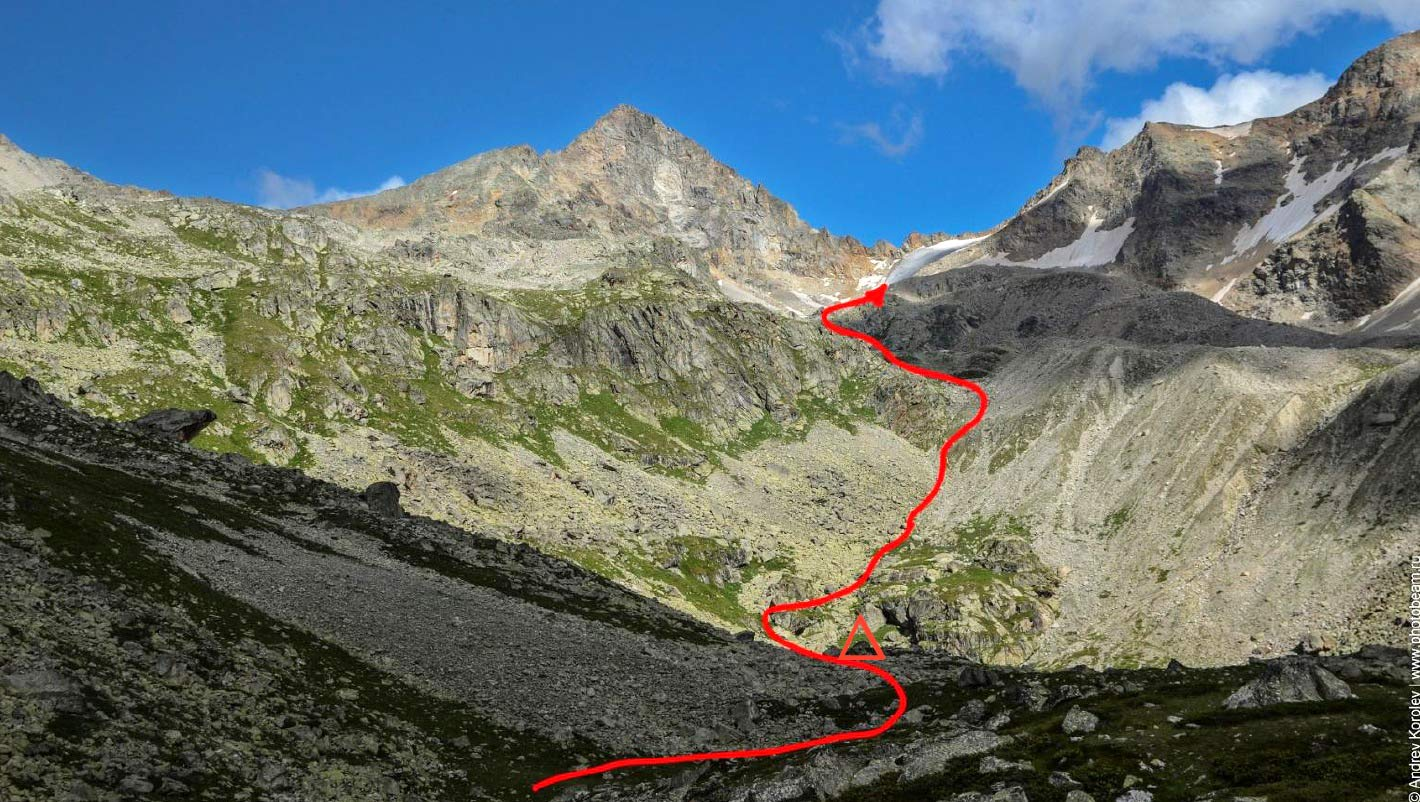
\includegraphics[angle=0, width=0.7\linewidth]{../pics/23augstart}
	\caption{Путь подъёма к перевалу Джалпаккол Северный от места ночёвки. Фото из отчёта Королёва А.Э. \cite{Korolyov2018}}
	\label{fig:23augstart}
\end{figure}

 Далее путь проходит по гребню моренного вала по слабомаркированной турами тропе. Путь утомительній, но физически и технически несложный. В 13:16 подходим под перевальный взлёт. Снега практически нет, ледник полностью открыт (рис.~\ref{fig:dzh_1}). Принимаем решение двигаться по правому пхд борту ледника. Как оказалось позднее, стандартный путь на этот перевал в виде <<крюка>> проходит ещё правее, но в нашем случае, когда снега на перевале не было, он проходил бы по осыпи, что только затруднило бы движение.
 



\begin{figure}[h!]
	\centering
	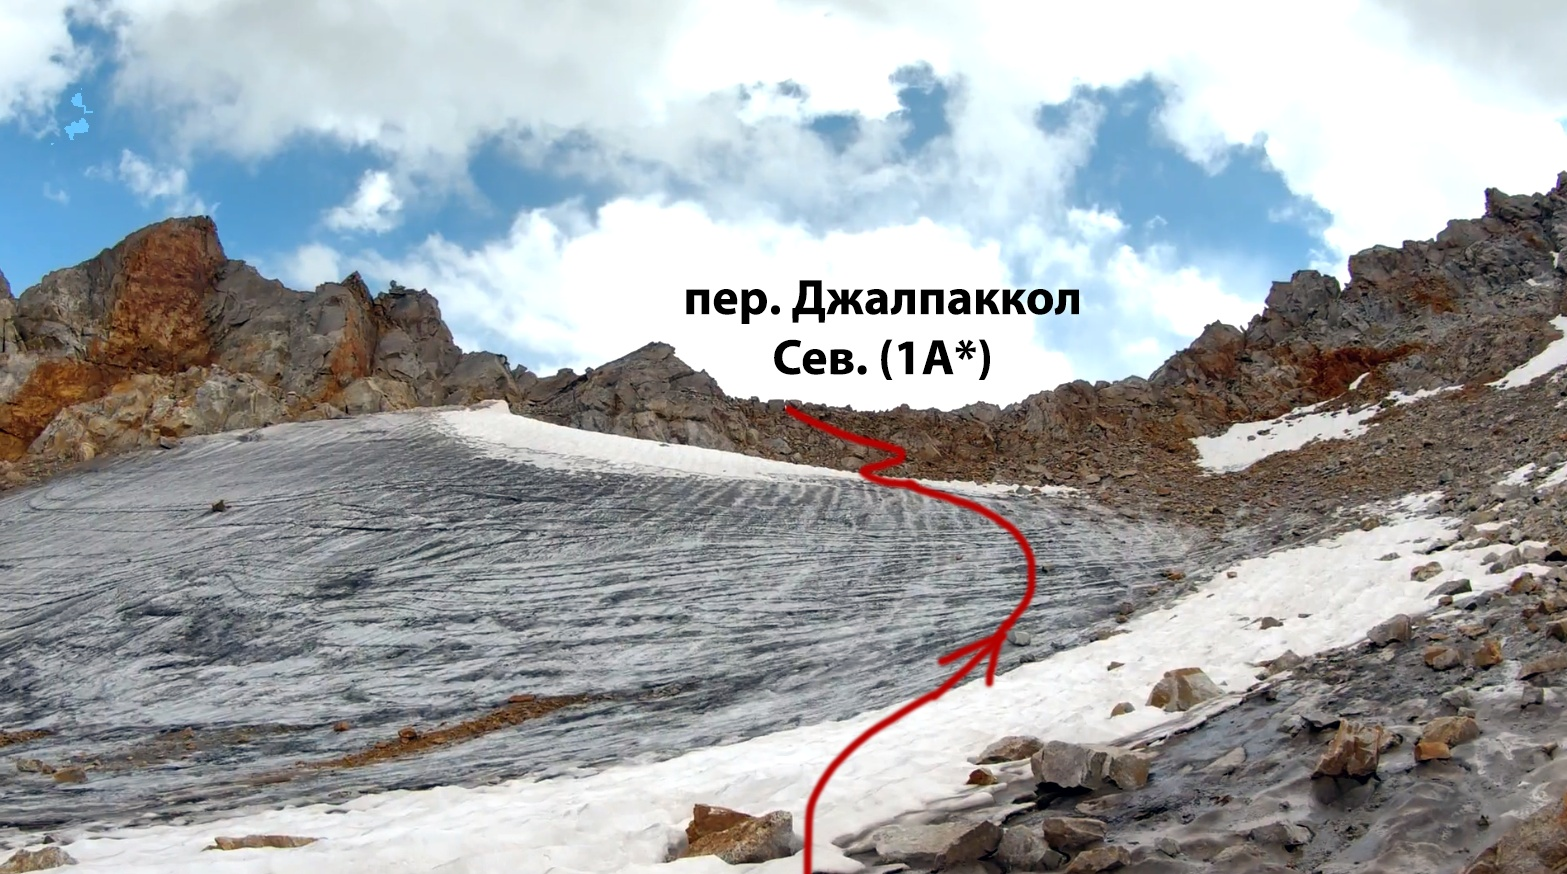
\includegraphics[width=0.7\linewidth]{../pics/dzh_1}
	\caption{Перевальный взлёт пер. Джалпаккол Северный}
	\label{fig:dzh_1}
\end{figure}

\begin{figure}[h!]	
	\centering
	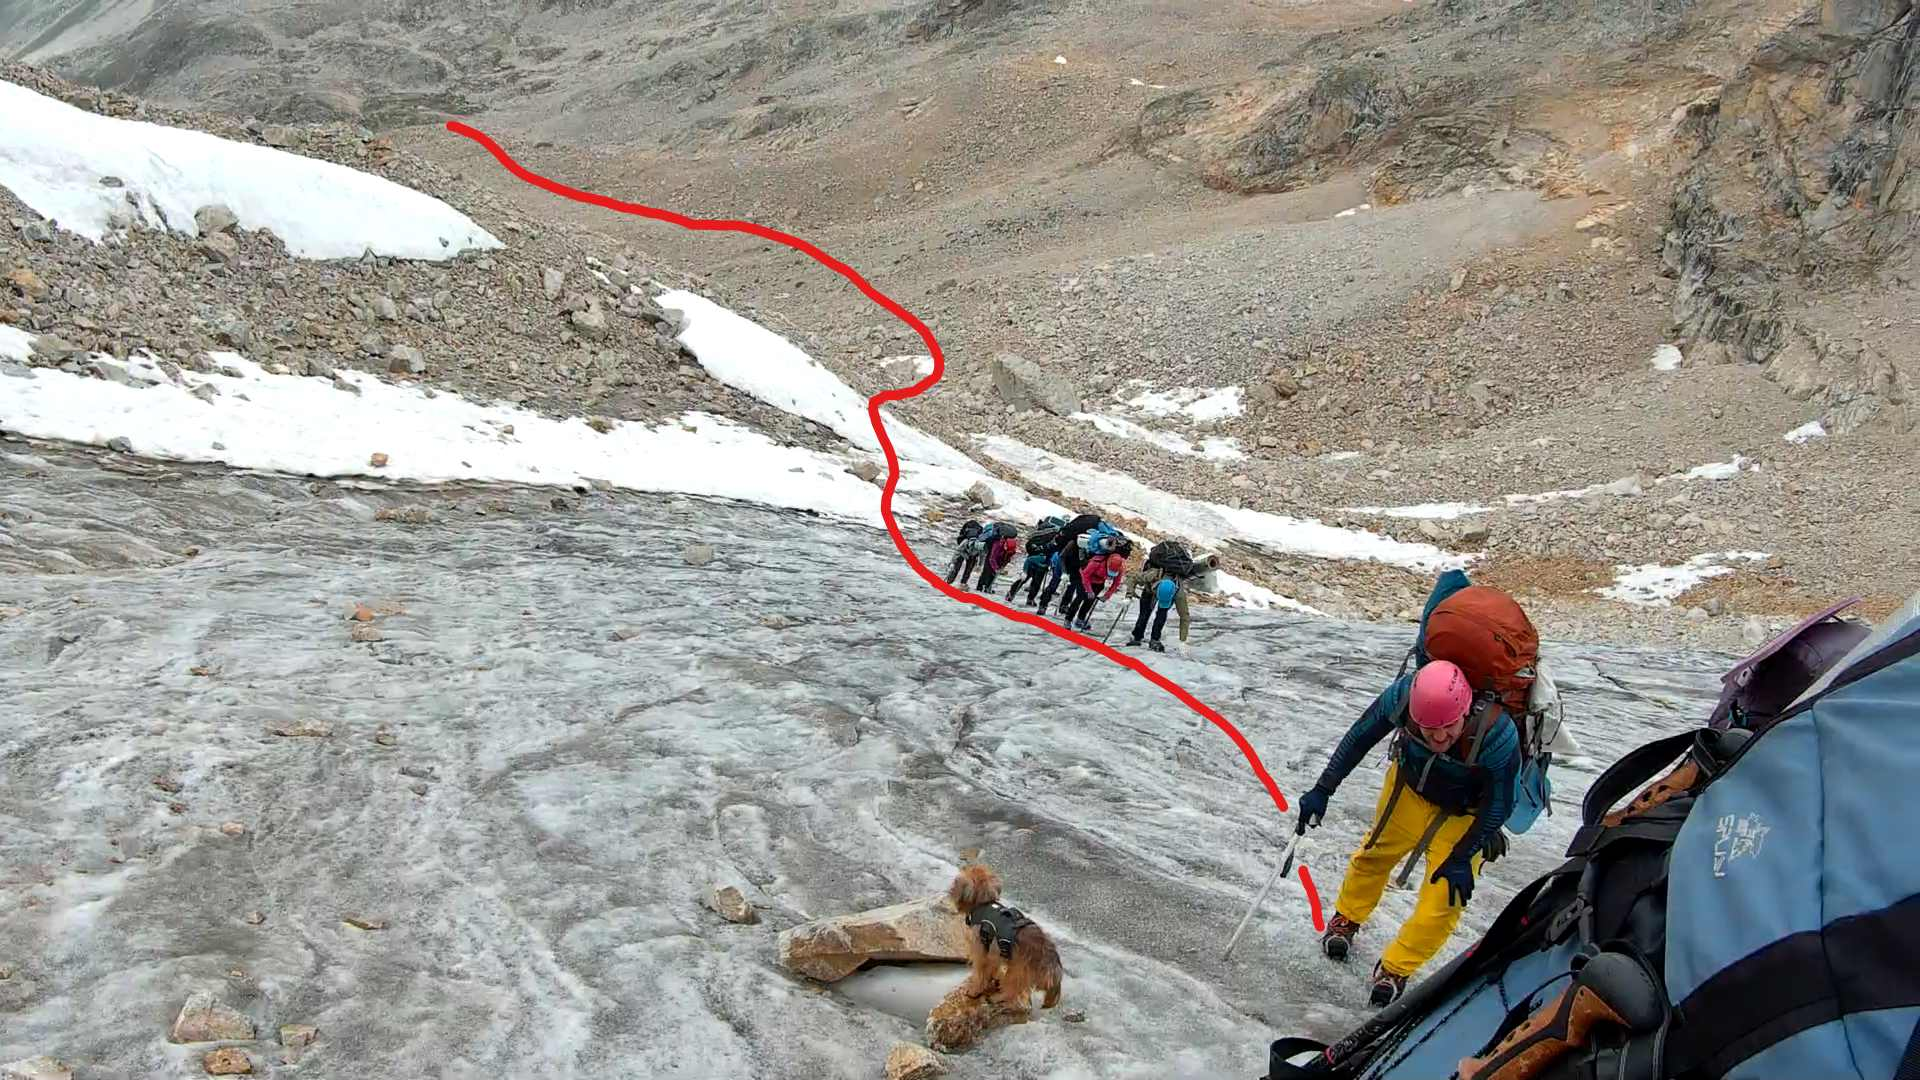
\includegraphics[angle=0, width=0.7\linewidth]{../pics/gopro_dzh}
	\caption{Подъём по леднику}
	\label{fig:gopro_dzh}
\end{figure}

\begin{figure}[h!]	
	\centering
	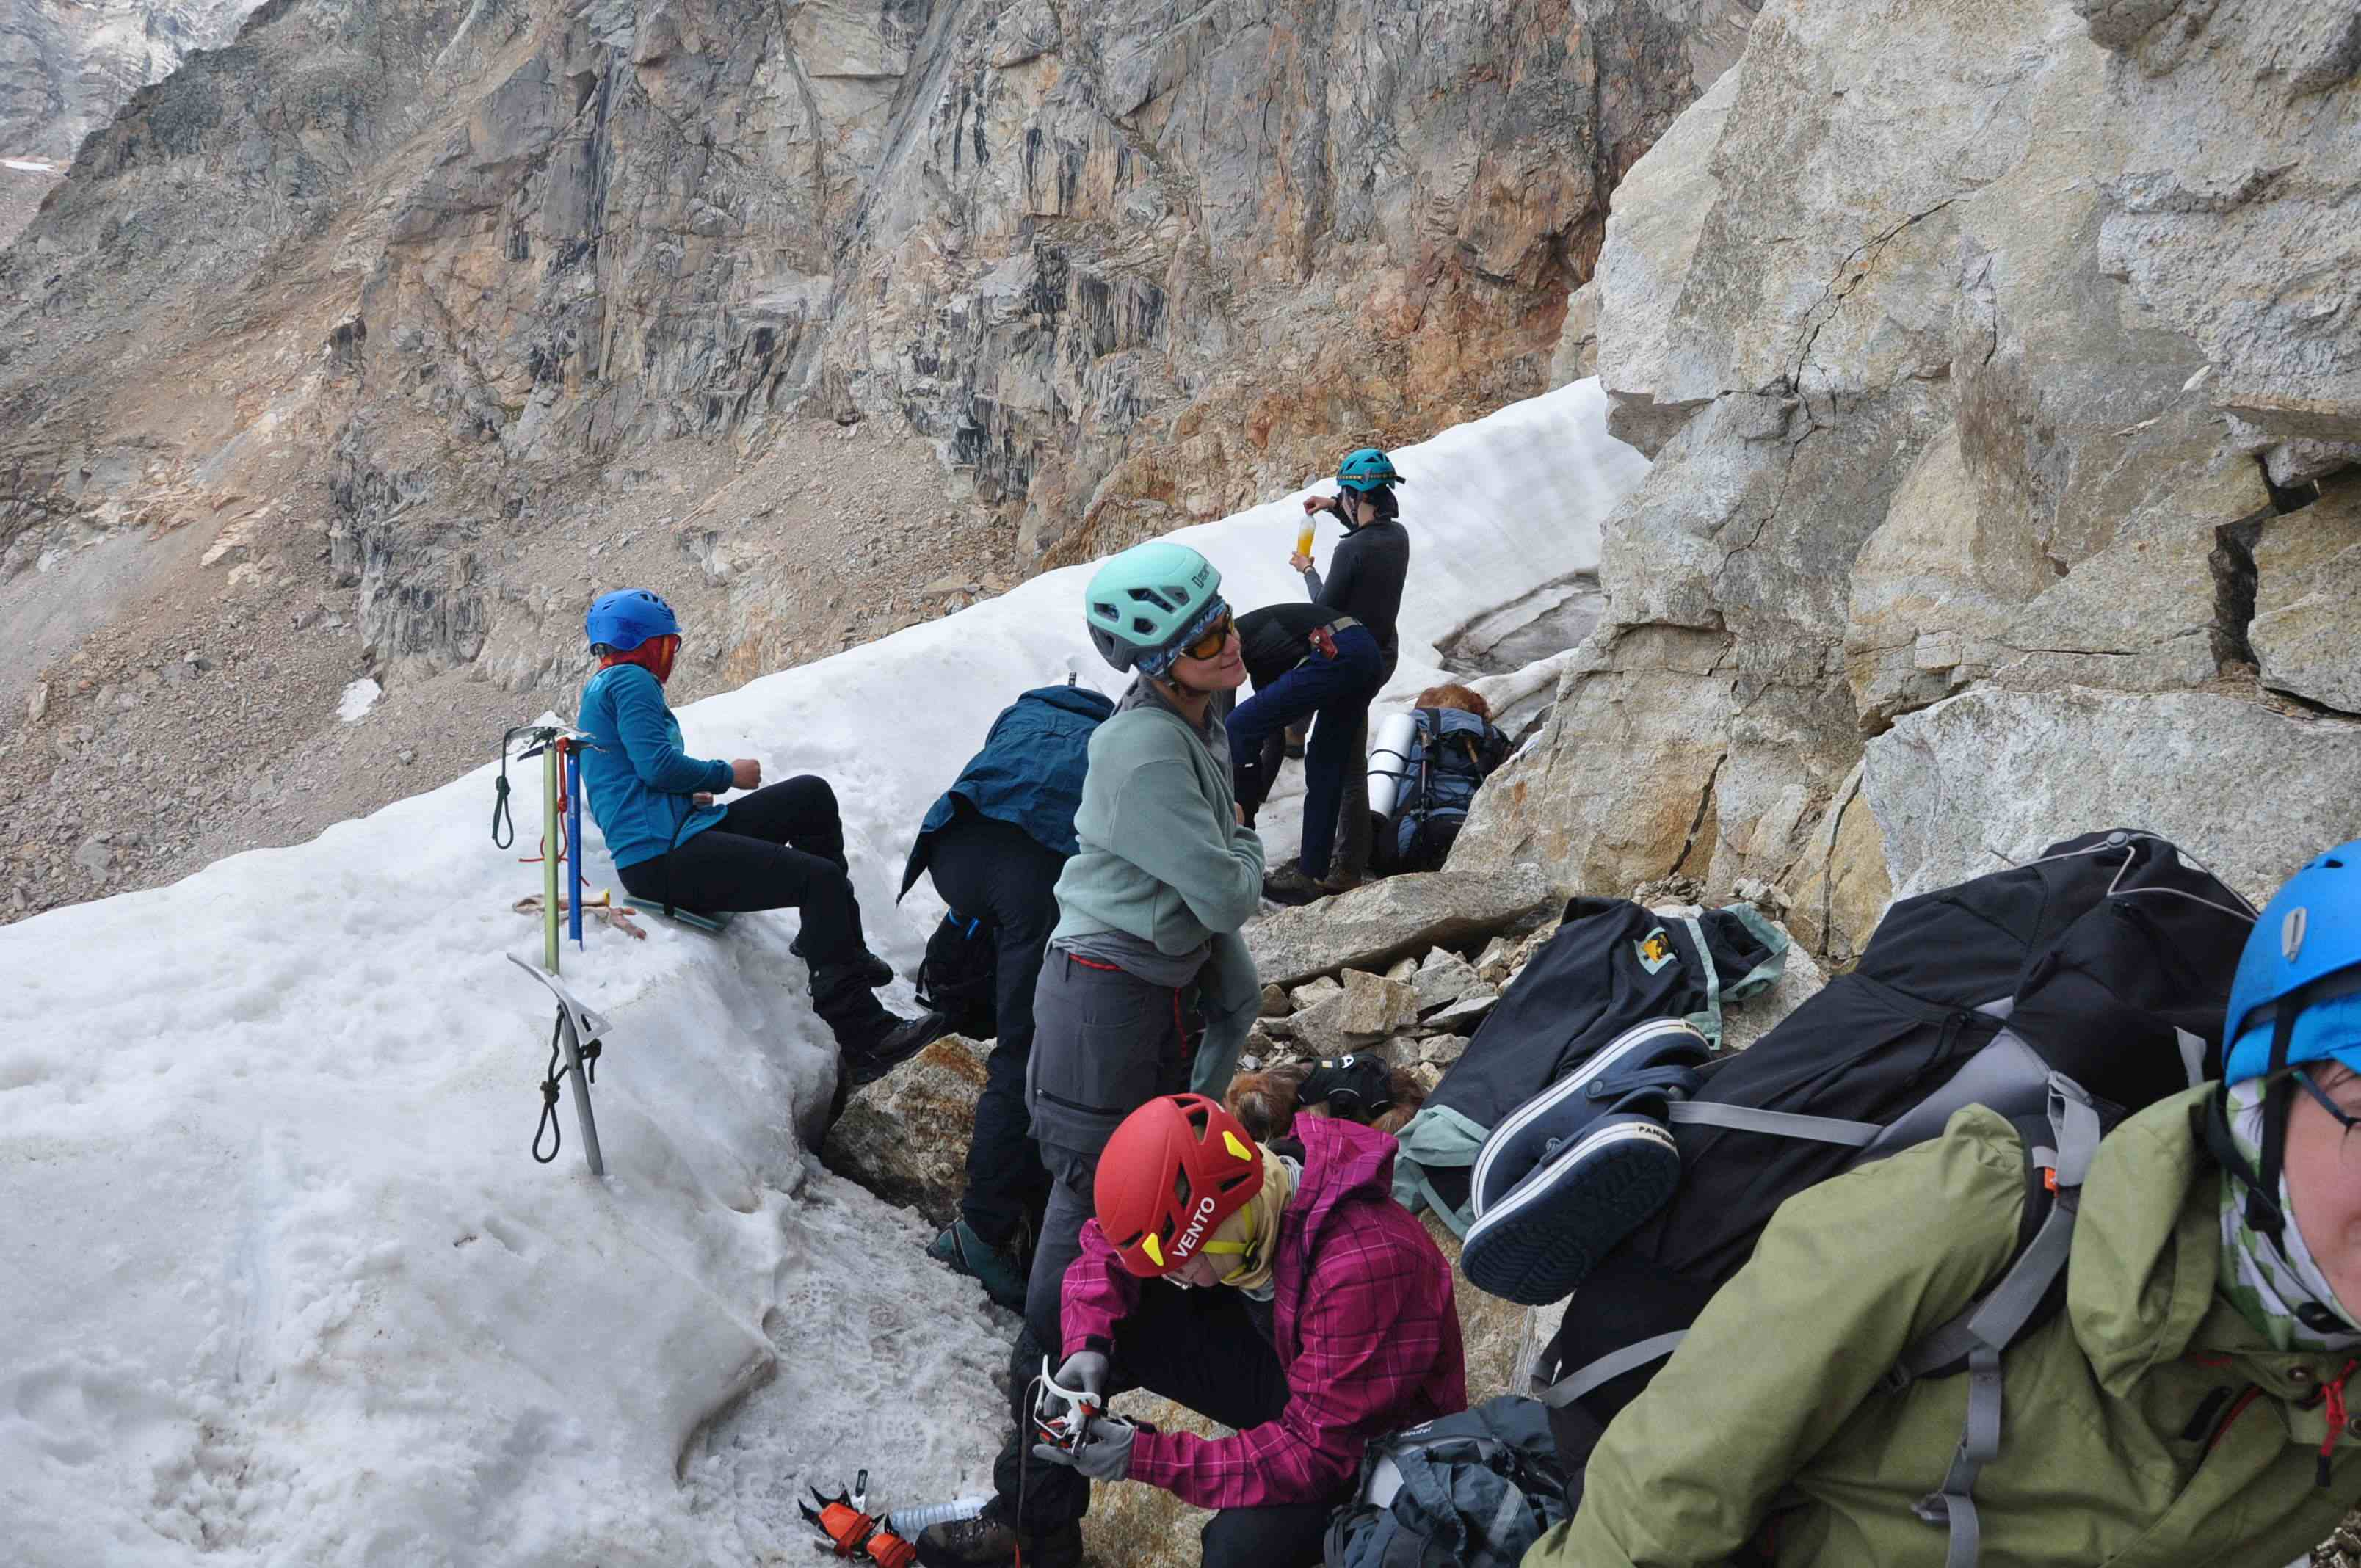
\includegraphics[angle=0, width=0.7\linewidth]{../pics/DSC_0021}
	\caption{Группа перед скальным участком перевала}
	\label{fig:DSC_0021}
\end{figure}








Подъём по леднику занимает 20 минут (рис.~\ref{fig:gopro_dzh}), в 14:45 приходим под финальный участок перевала~--- 10 метров лазания по сильно разрушенным скалам (рис.~\ref{fig:DSC_0021}) и снимаем кошки.

Руководитель идёт на разведку без рюкзака, после чего группа командами по 2-3 человека поднимается на седловину. В 15:30 вся группа оказывается на перевале (рис.~\ref{fig:DSC_0063}, \ref{fig:DSC_0069}).

\begin{figure}[h!]	
	\centering
	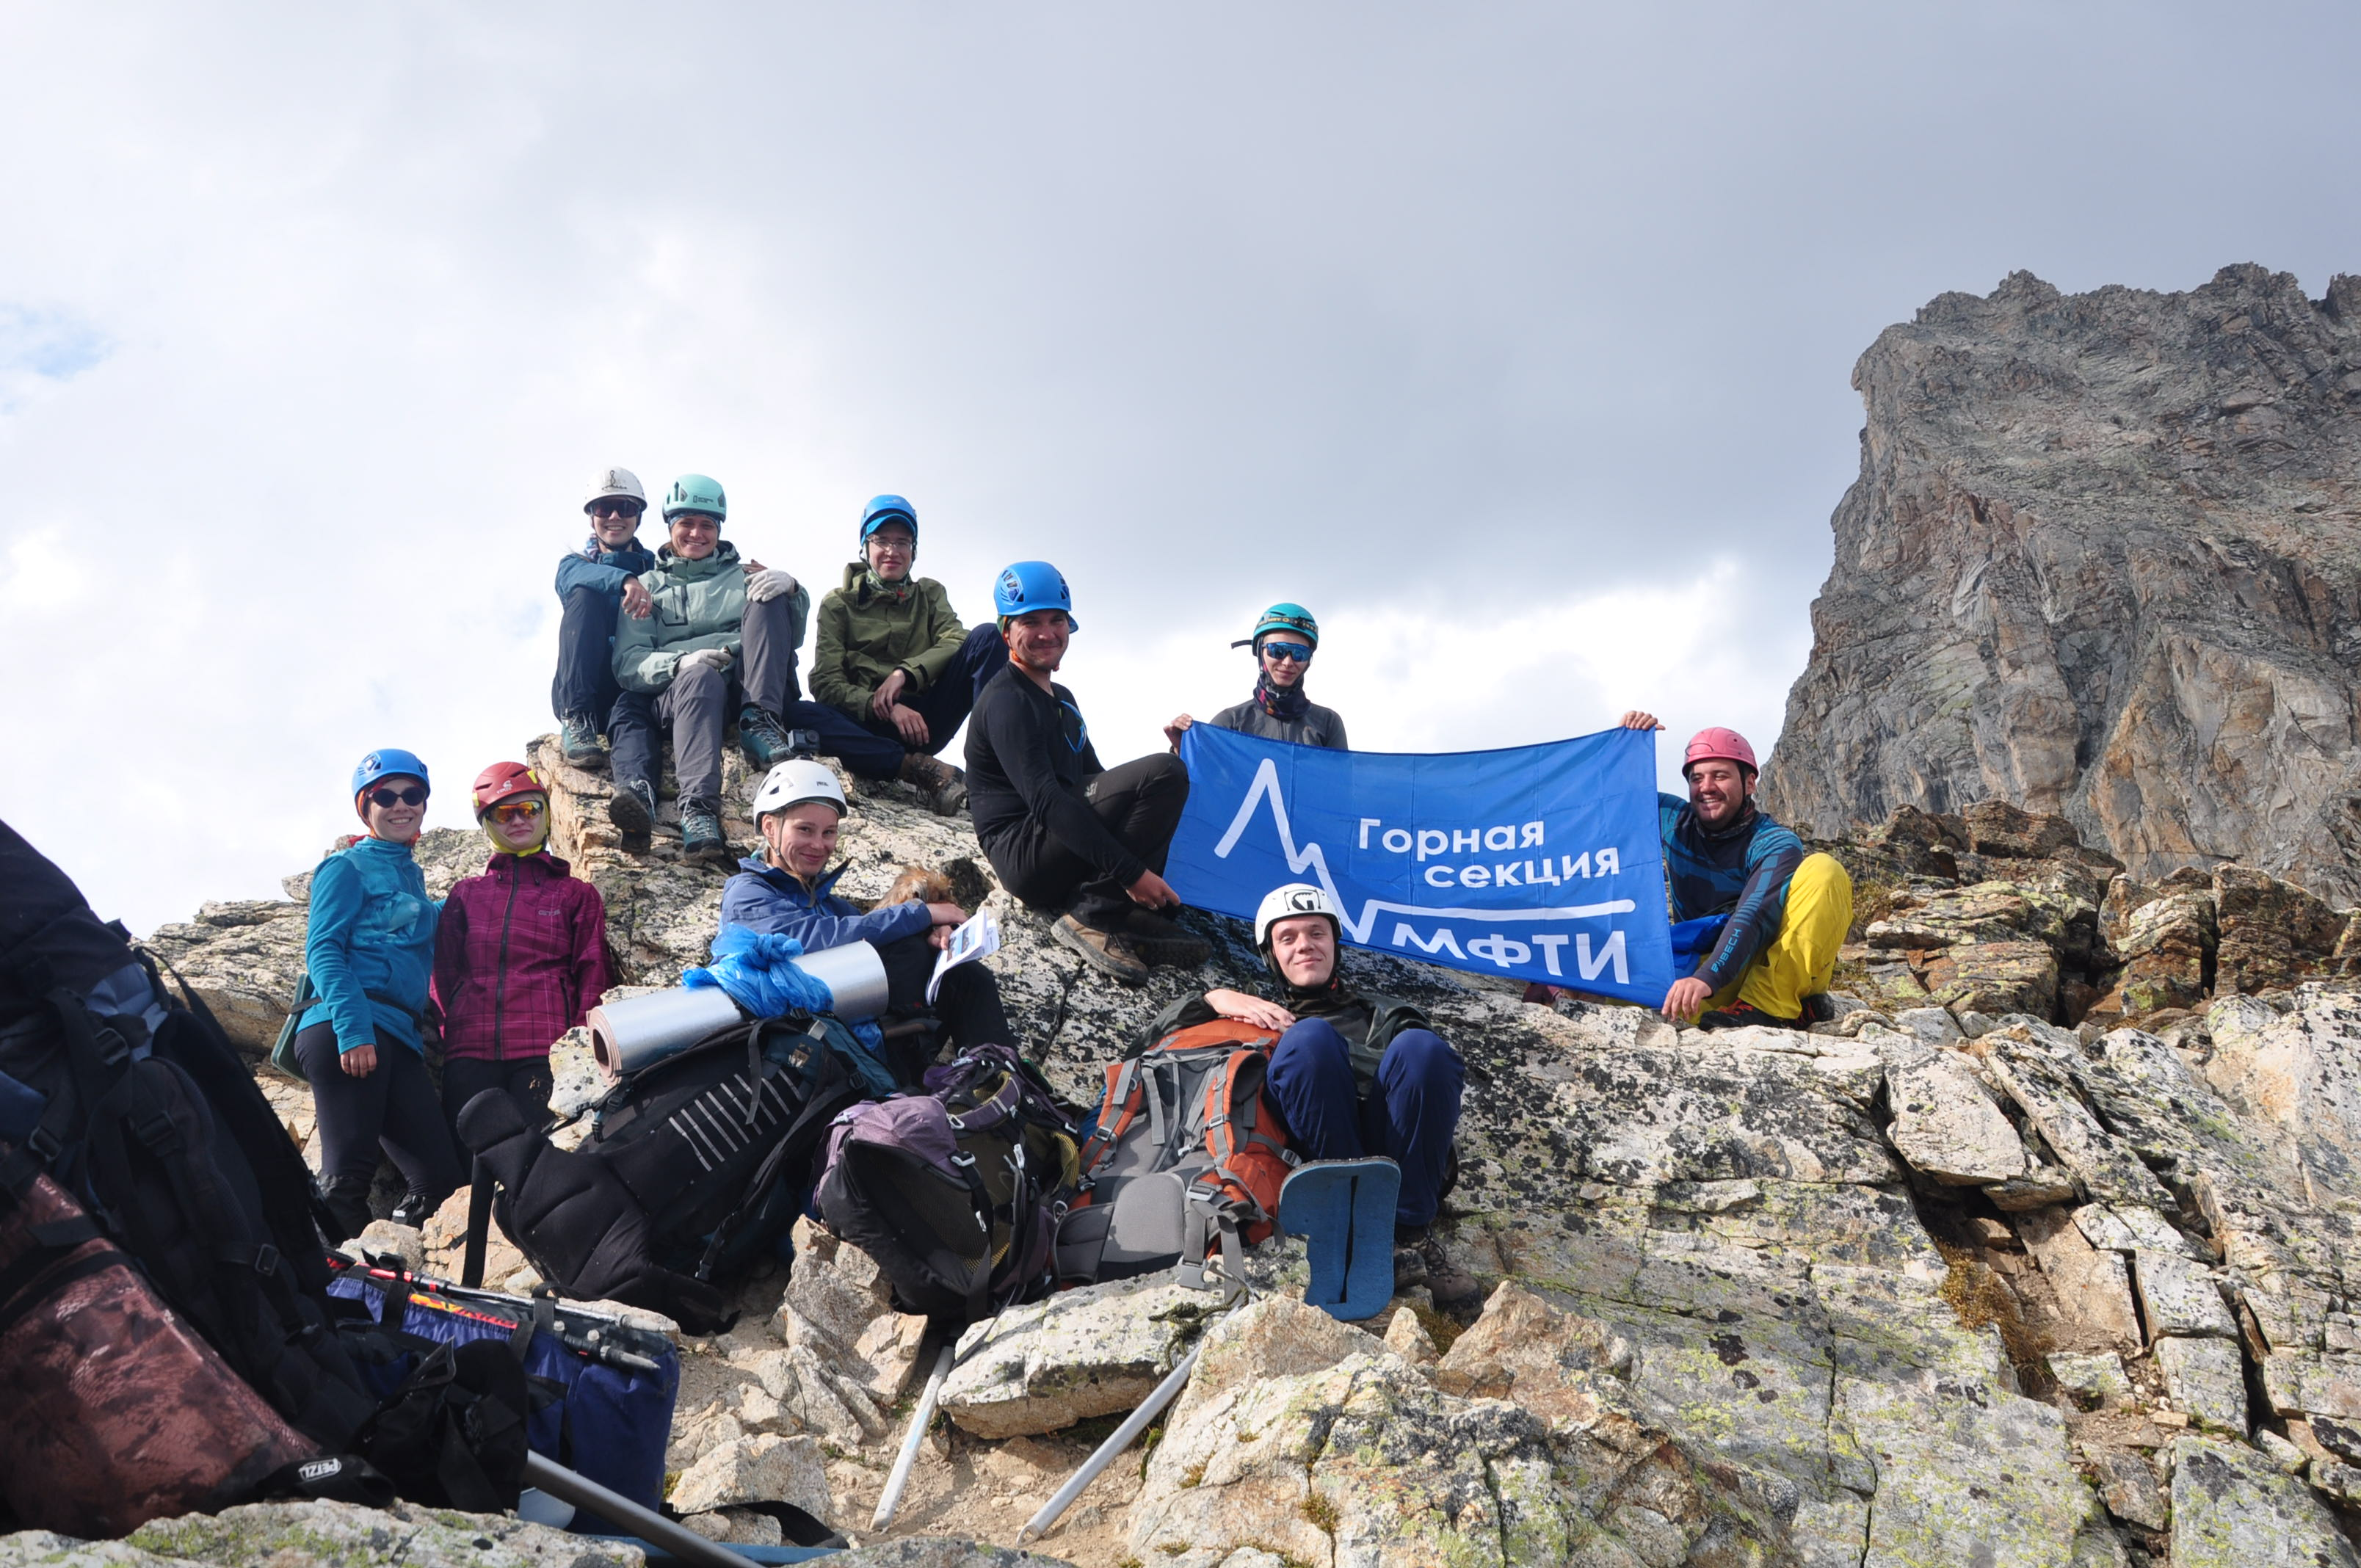
\includegraphics[angle=0, width=0.7\linewidth]{../pics/DSC_0063}
	\caption{Группа на пер. Джалпаккол Северный (1А$^\star$)}
	\label{fig:DSC_0063}
\end{figure}

\begin{figure}[h!]	
	\centering
	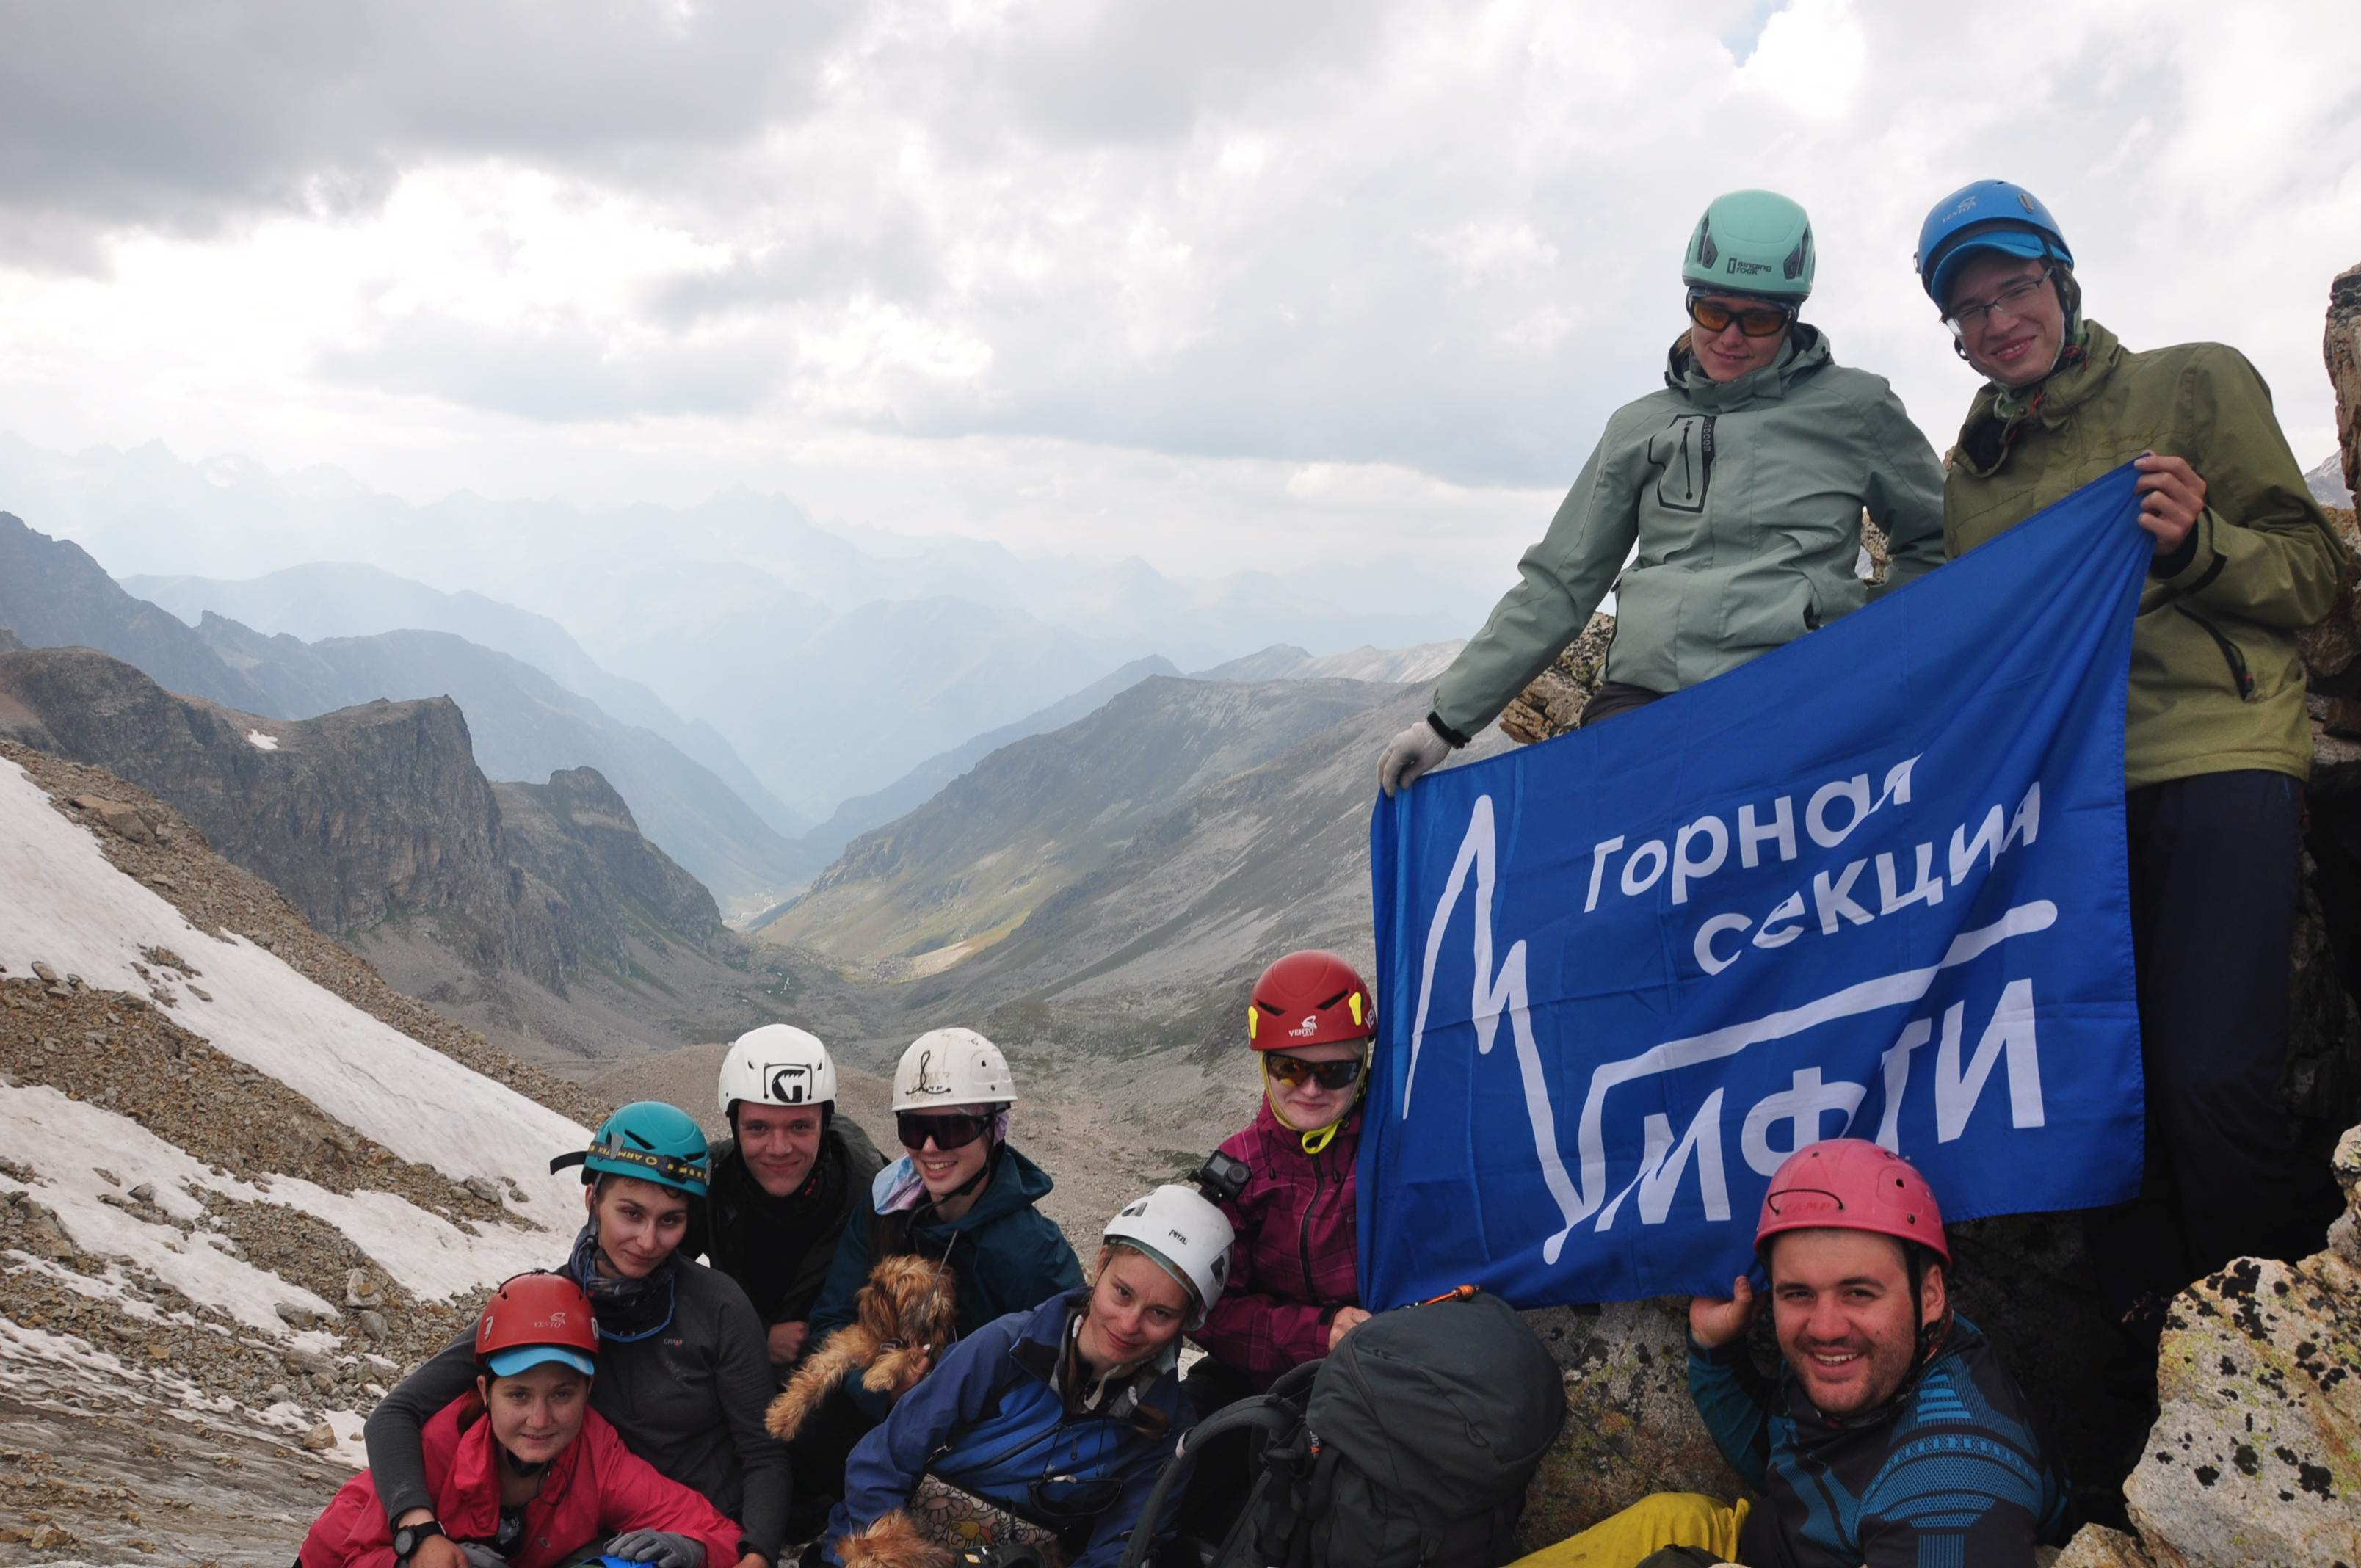
\includegraphics[angle=0, width=0.7\linewidth]{../pics/DSC_0069}
	\caption{Группа на пер. Джалпаккол Северный (1А$^\star$), вид в д.р. Кичкинекол Джалпаккольский}
	\label{fig:DSC_0069}
\end{figure}

\begin{figure}[h!]	
	\centering
	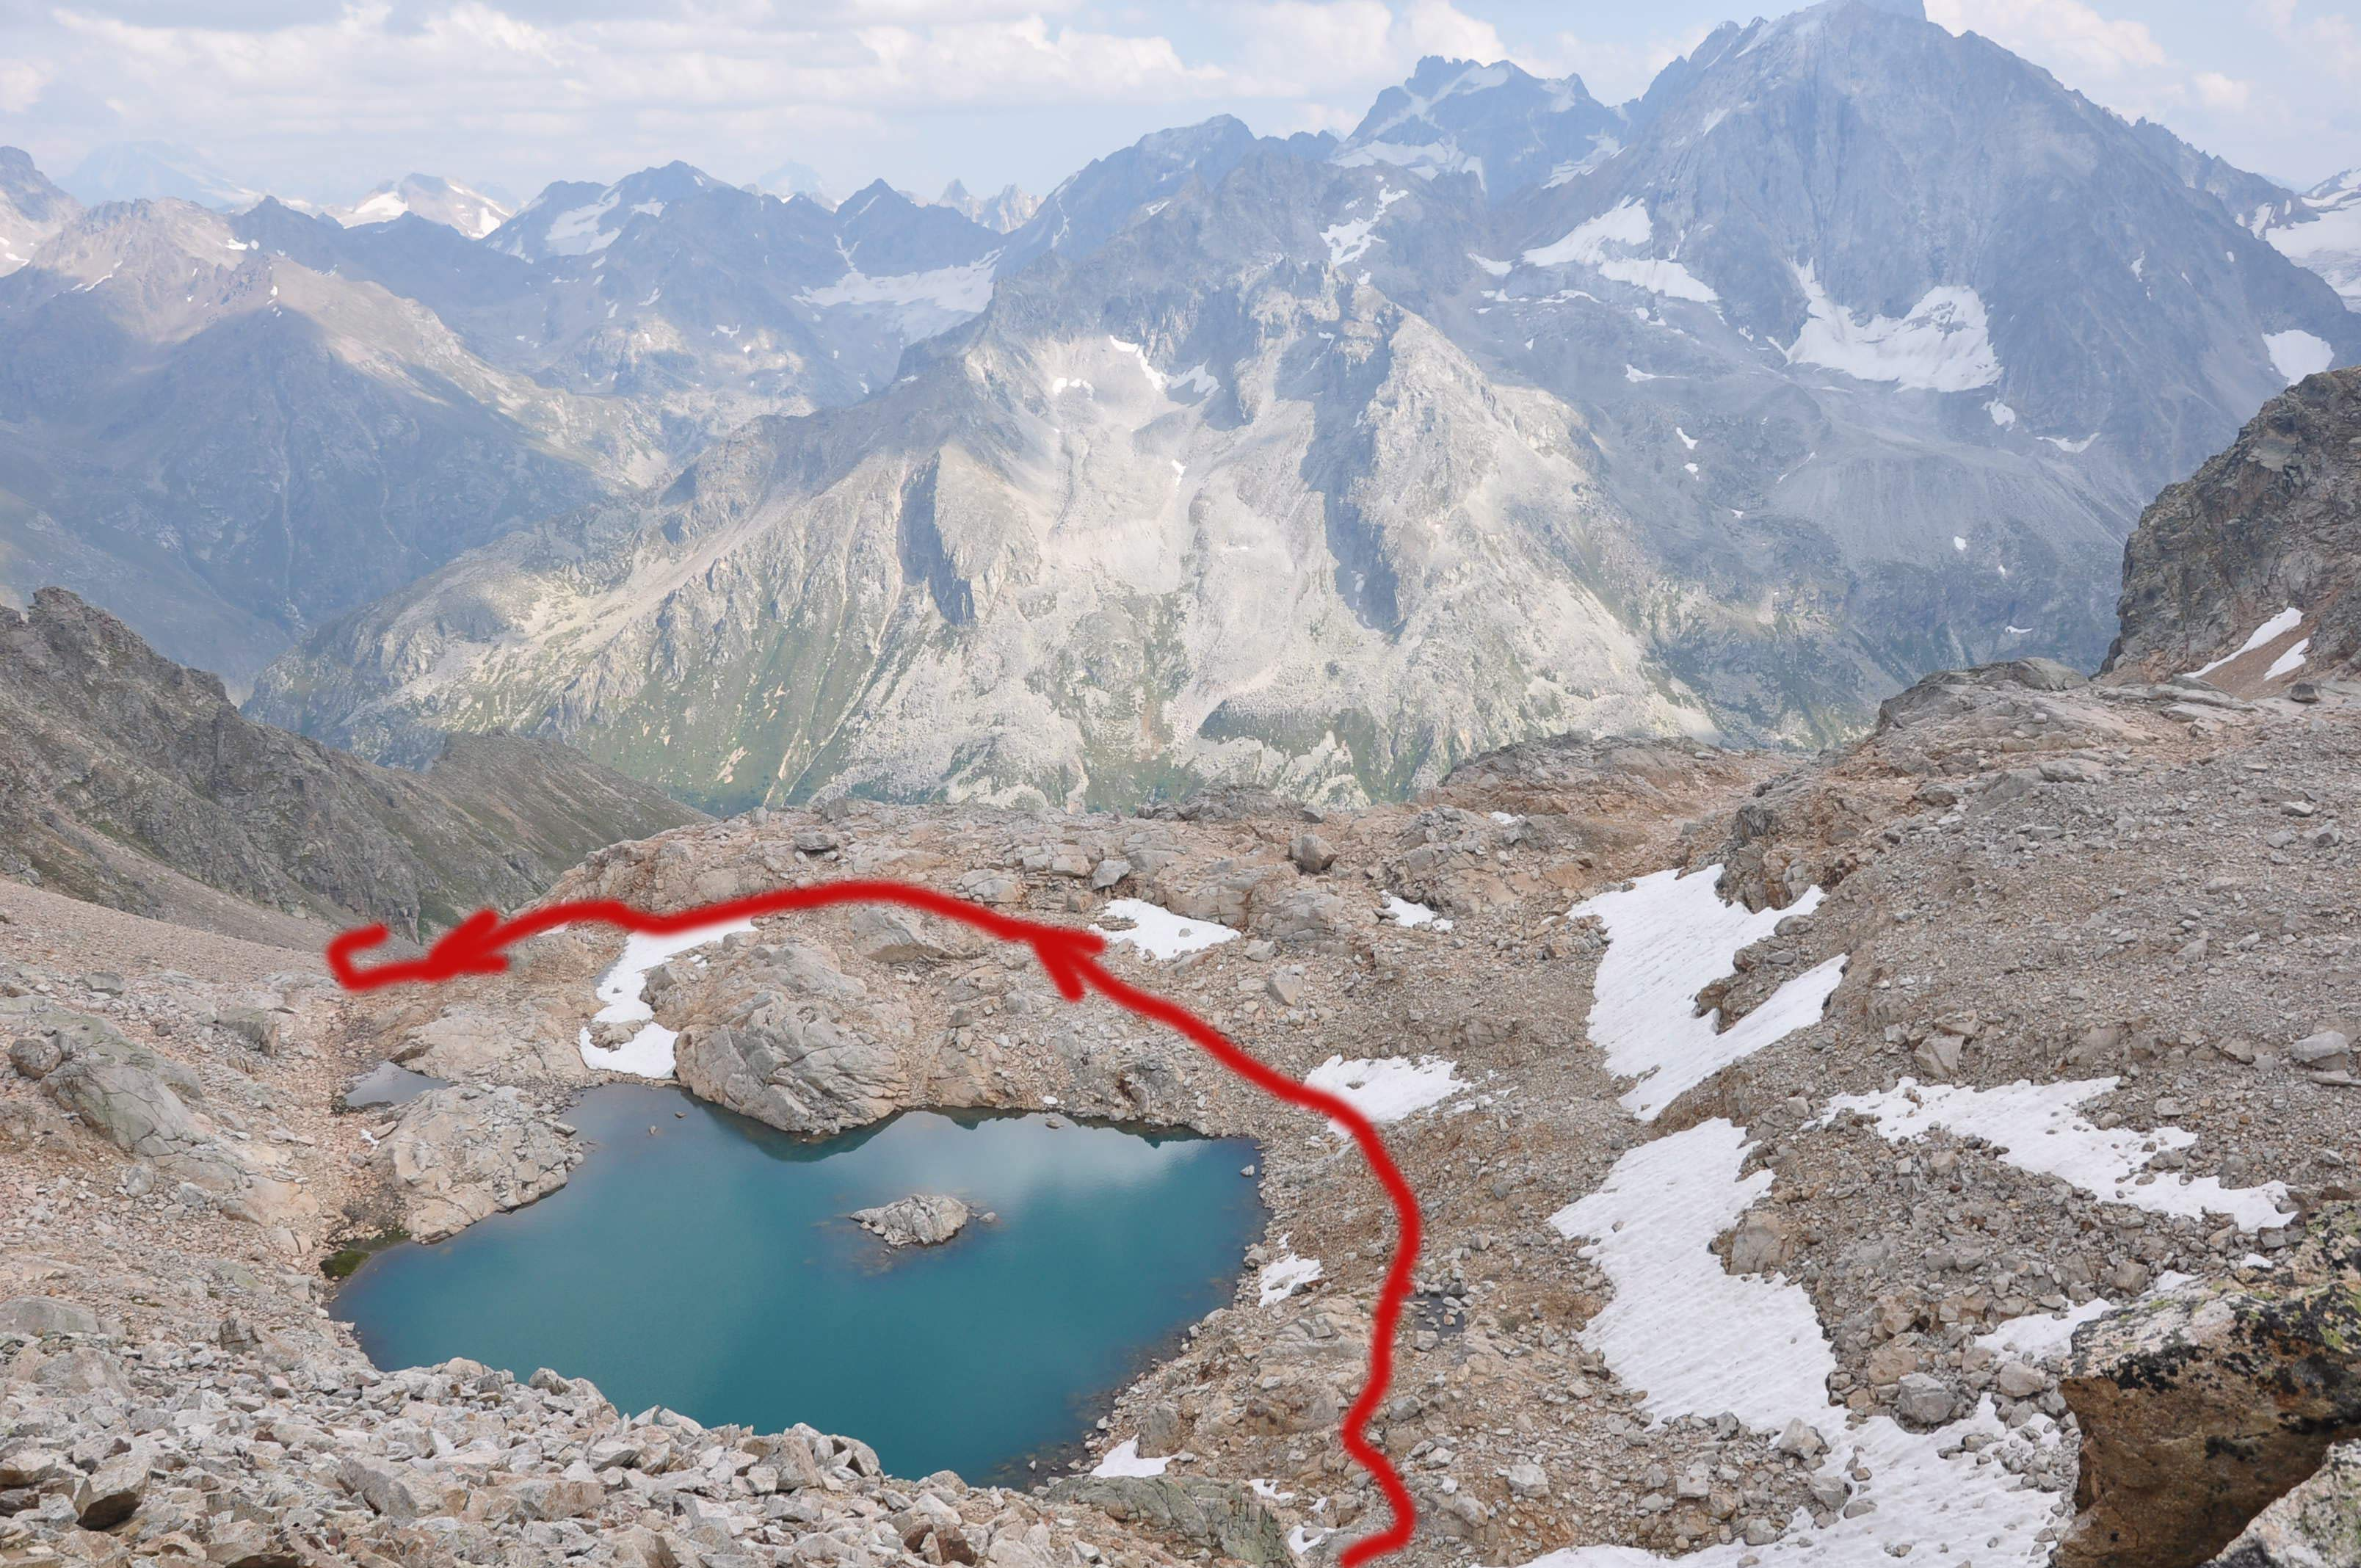
\includegraphics[angle=0, width=0.7\linewidth]{../pics/DSC_0041}
	\caption{Вид с перевала на спуск в д.р. Мырды}
	\label{fig:DSC_0041}
\end{figure}

В 16:15 начинаем спуск (рис.~\ref{fig:DSC_0041}), перевальный взлёт представляет собой среднюю и мелкую осыпь. К озеру под перевалом спускаемся в 17:00 и обходим его справа пхд (по южному берегу). Опускается туман, накрапывает мелкий дождь (рис.~\ref{fig:IMG_20240823_170306}). Бараньи лбы на восточной оконечности озера и далее по спуску проходим максимально аккуратно, так как от дождя камни стали скользкими.
 
\begin{figure}[h!]	
	\centering
	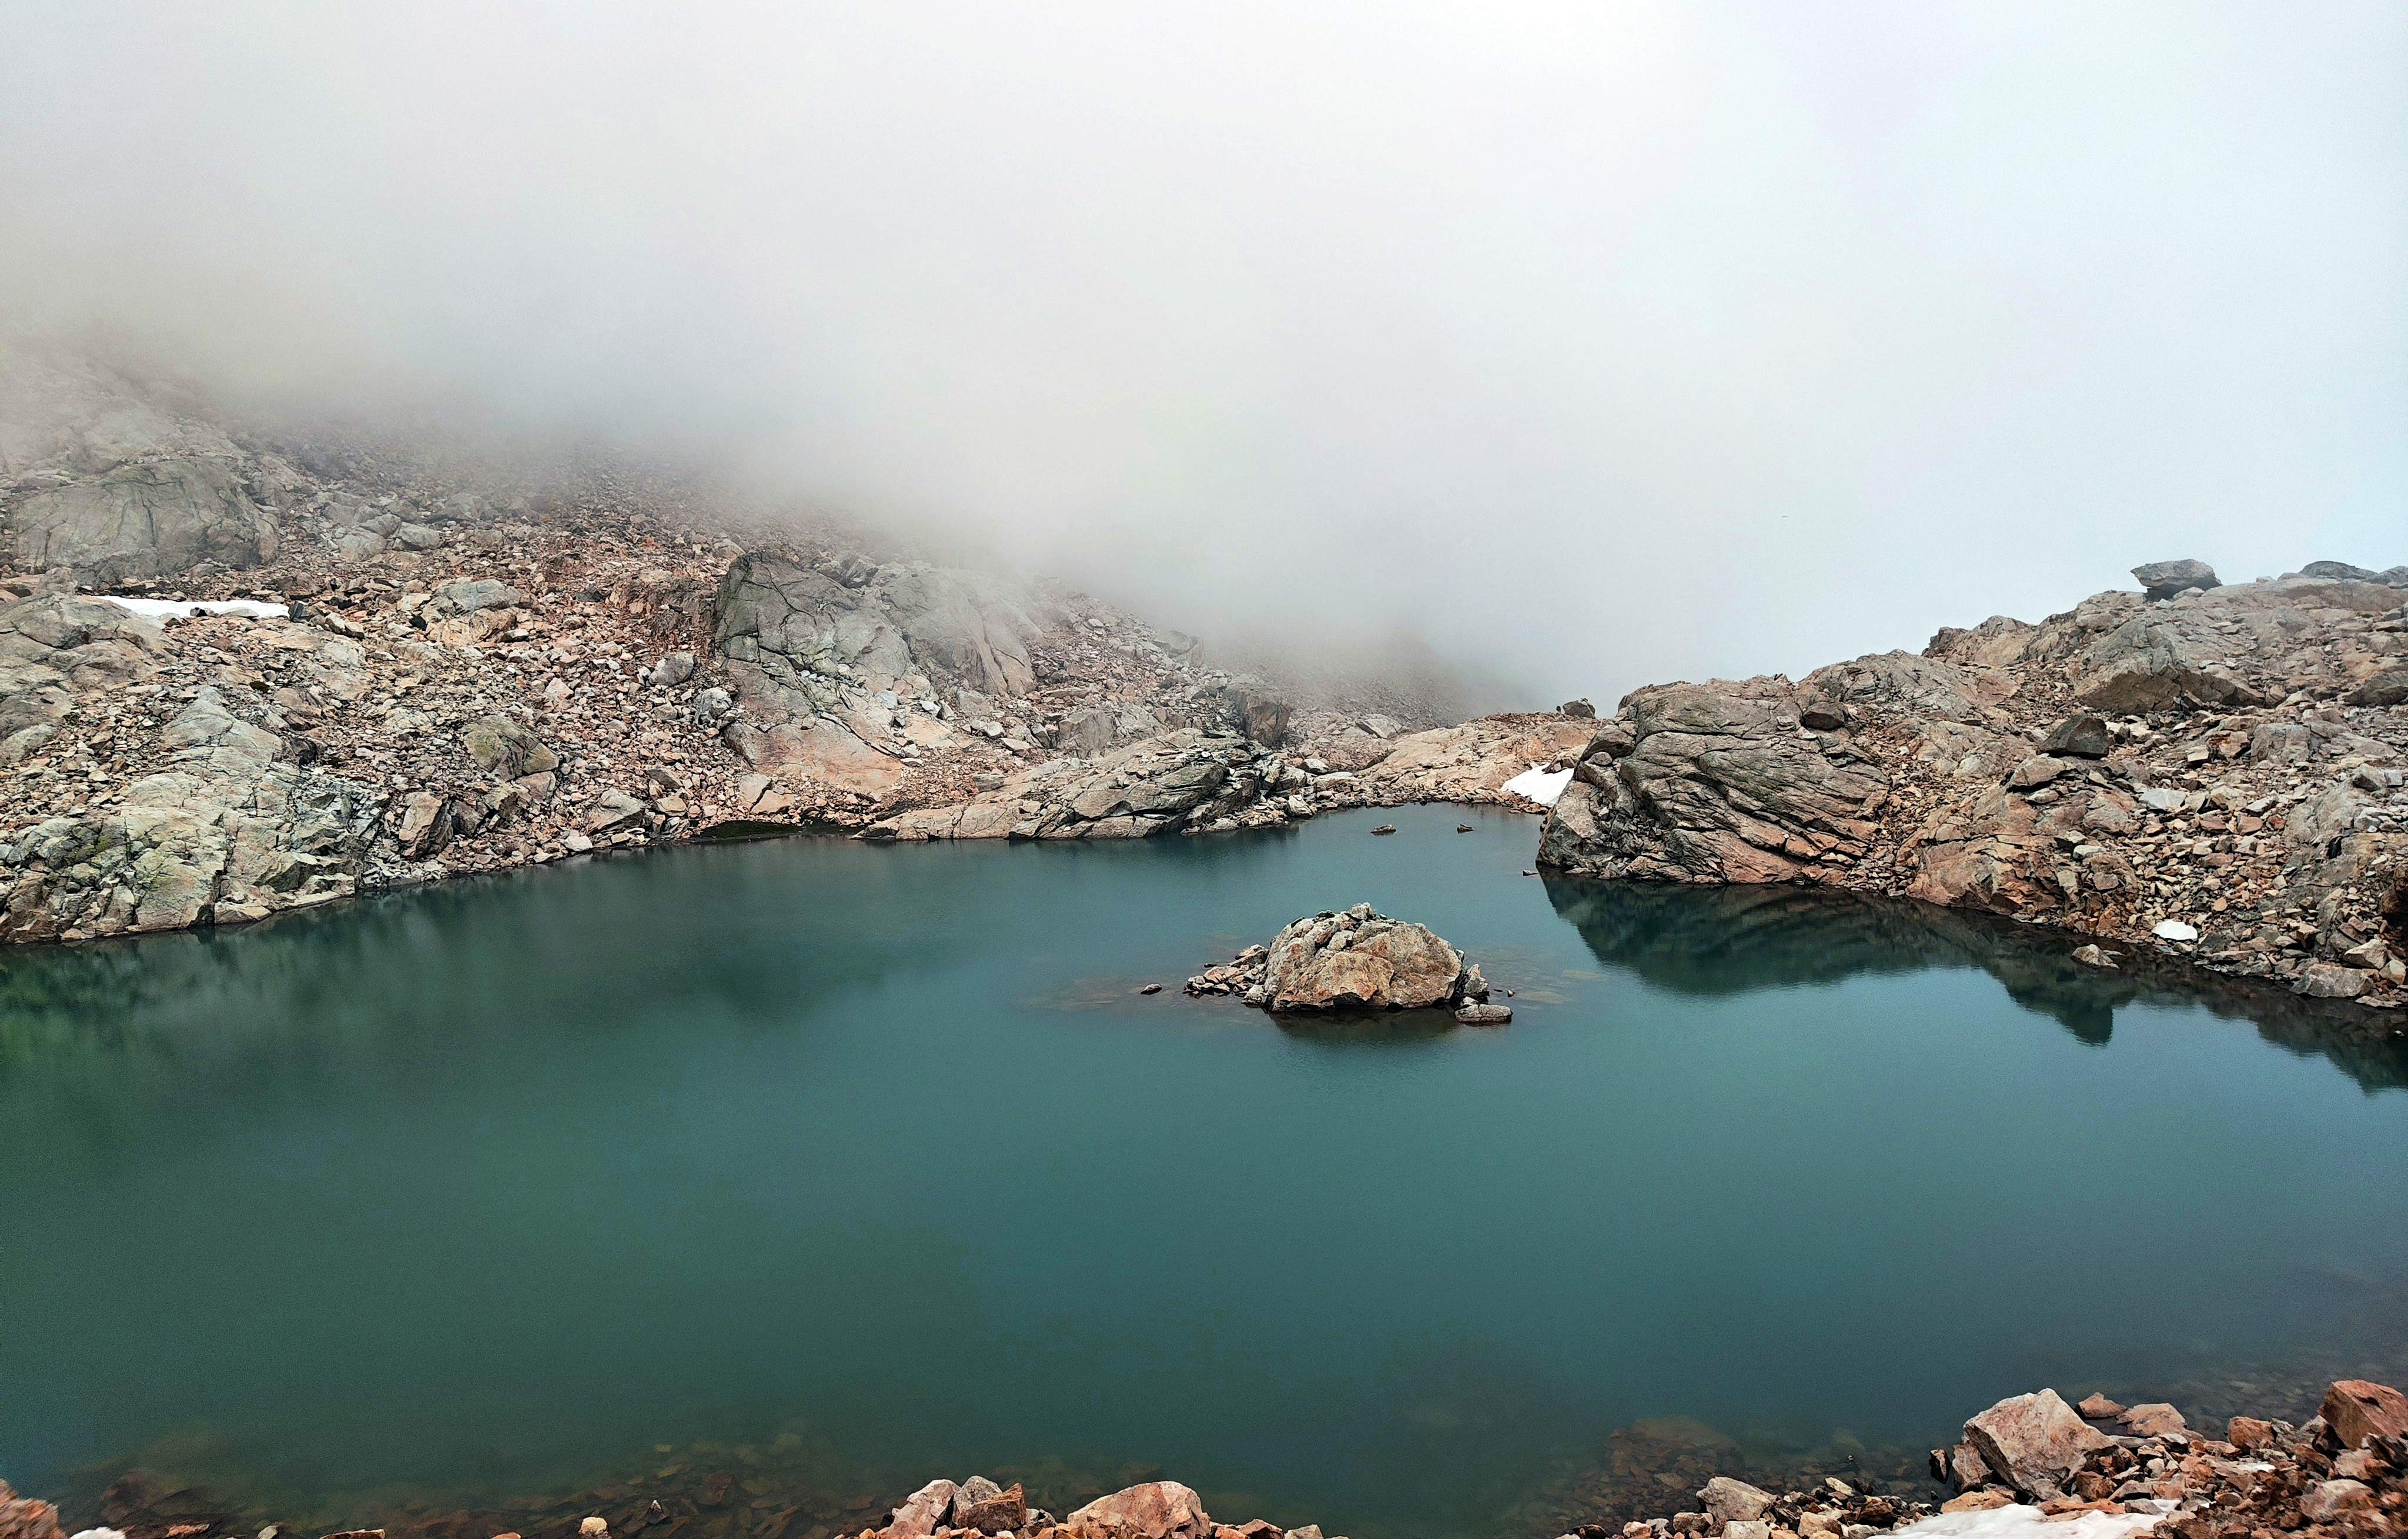
\includegraphics[angle=0, width=0.7\linewidth]{../pics/IMG_20240823_170306}
	\caption{Туман на озере под пер. Джалпаккол Северный}
	\label{fig:IMG_20240823_170306}
\end{figure}

В 18:30 спускаемся на оборудованные стоянки на выполаживании травянисто-осыпного склона (рис.~\ref{fig:IMG_20240823_184041}). Координаты м.н.: N~43.274531\degree, E~42.122488\degree.

\begin{figure}[h!]	
	\centering
	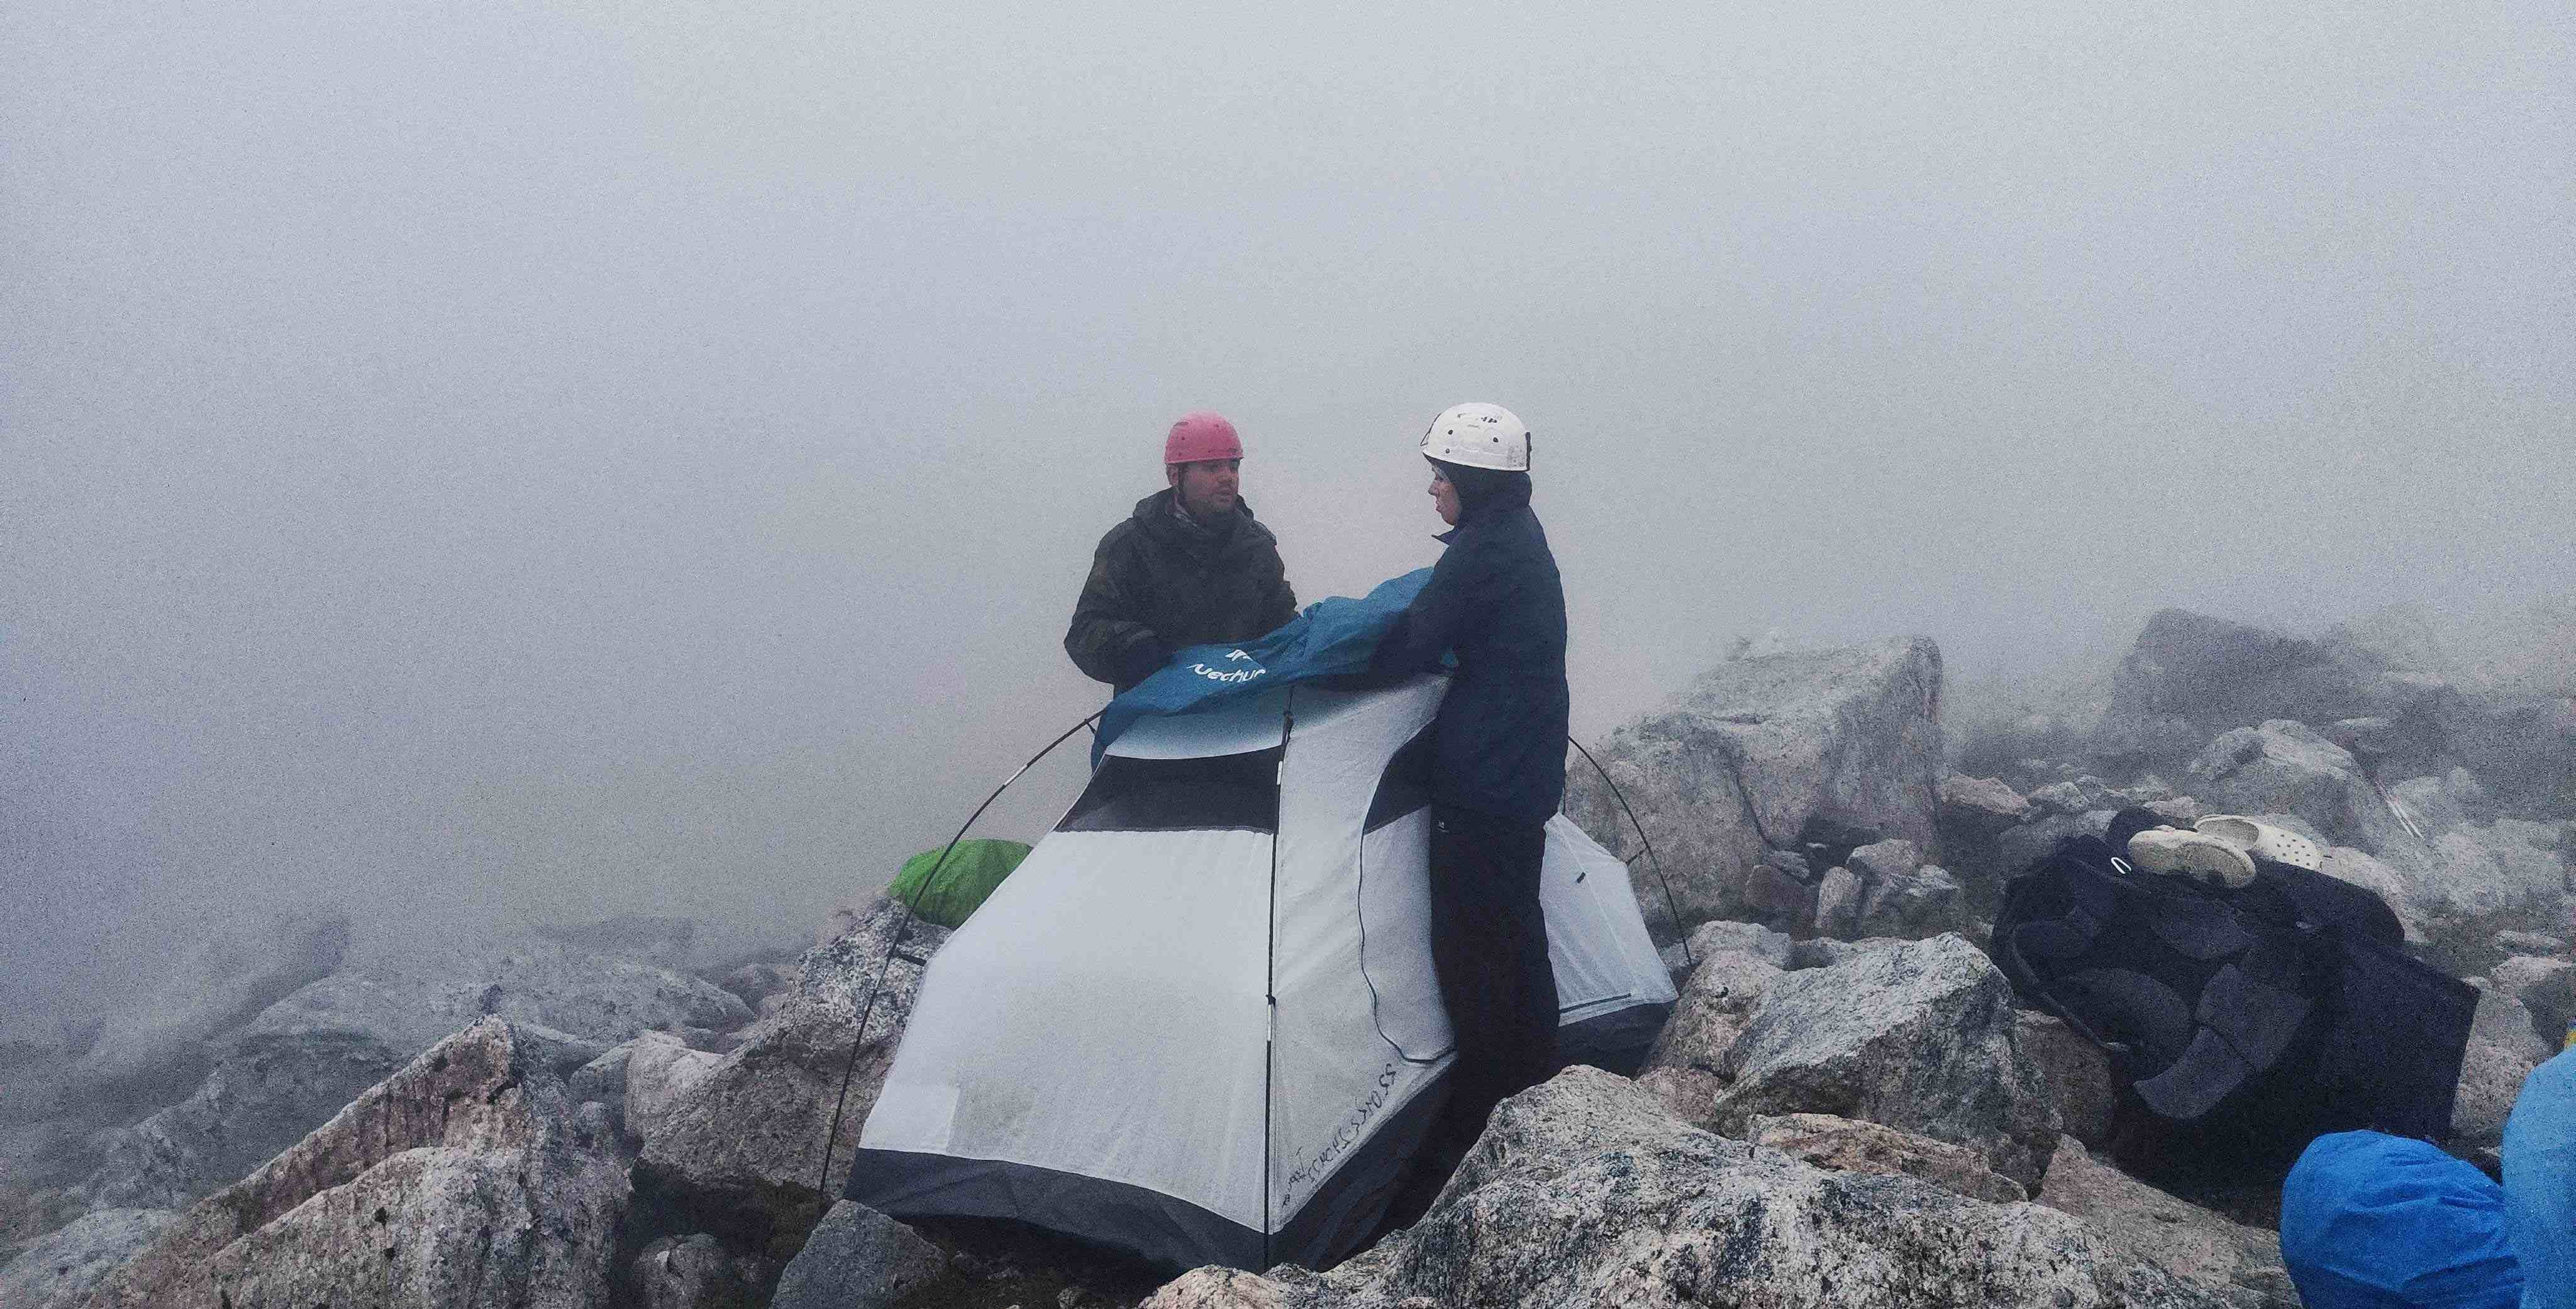
\includegraphics[angle=0, width=0.7\linewidth]{../pics/IMG_20240823_184041}
	\caption{м.н. 23-24 августа}
	\label{fig:IMG_20240823_184041}
\end{figure}

 Высота ночёвки в этот день была максимальной за весь поход и составила 3050~м. Источника воды на месте не оказалось, так как озеро у площадок пересохло. Ближайший источник воды оказался в 200~м к западу от м.н., в также почти пересохшем озере, которое спряталось за локальной возвышенностью. Часть команды, которая ходила за водой, брала с собой навигатор и поддерживала связь с оставшимися в лагере туристами голосом, так как видимость в тумане не превышала 20~м.



\begin{figure}[h!]	
	\centering
	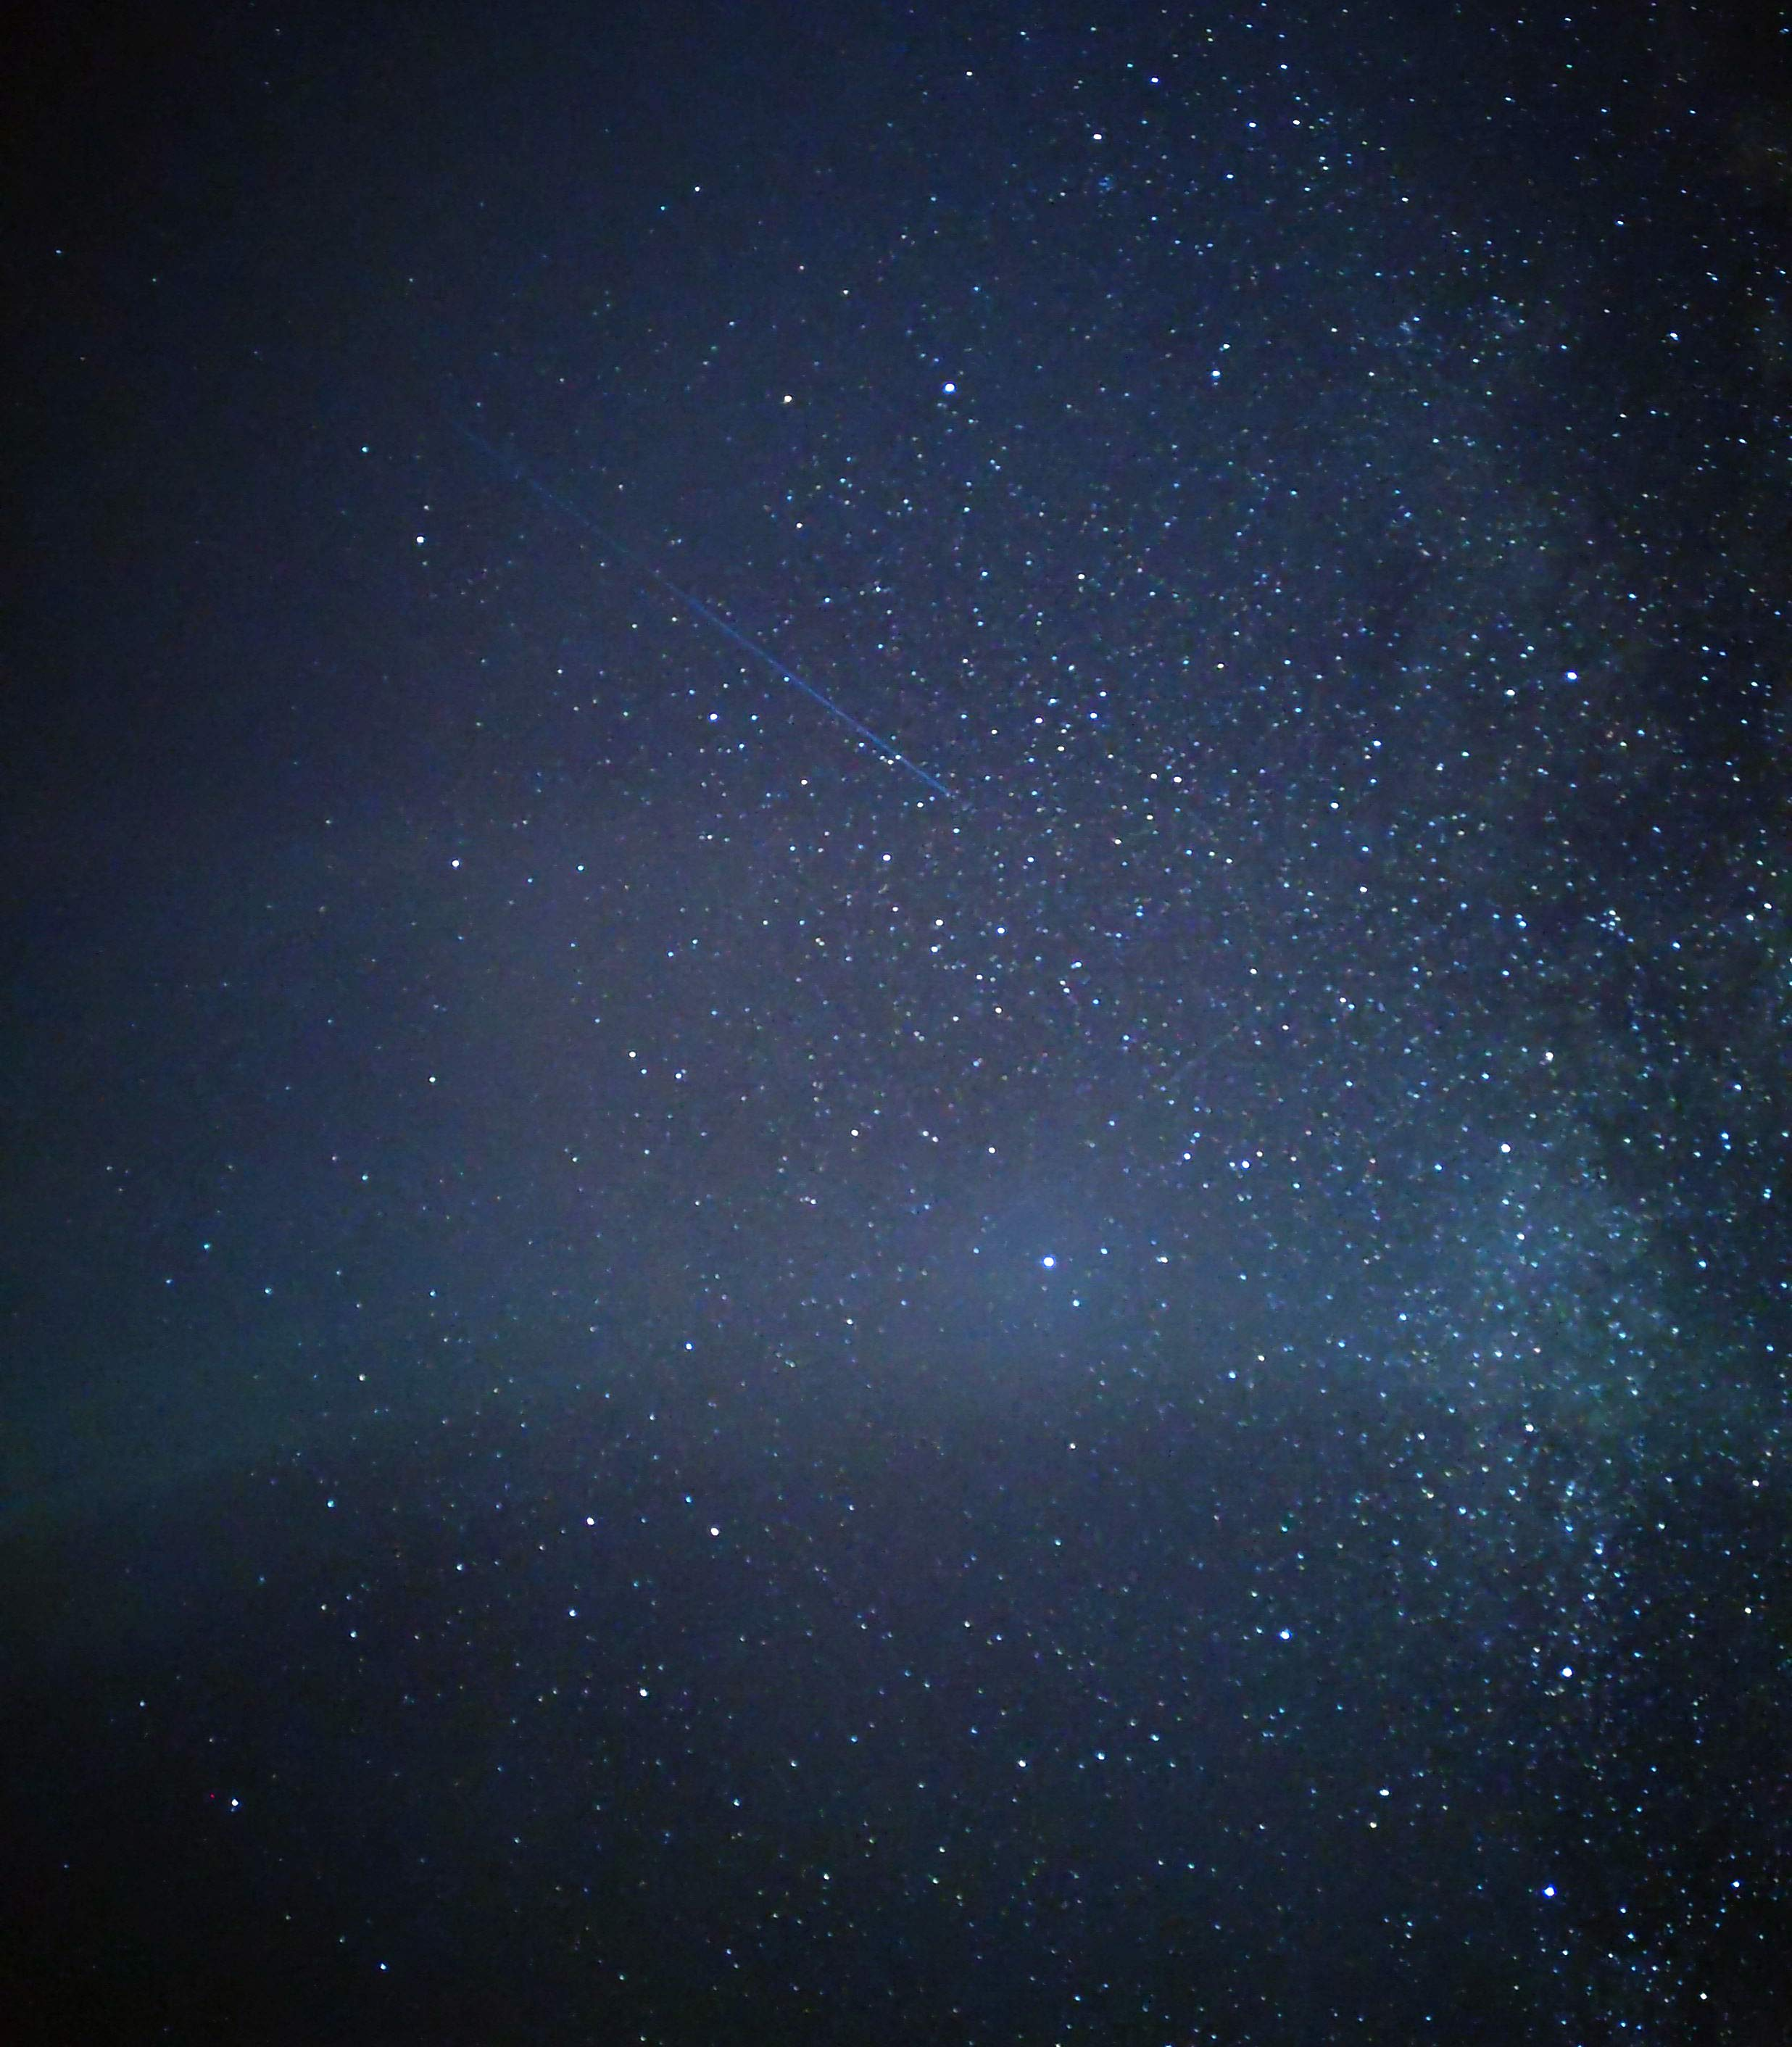
\includegraphics[angle=0, width=0.7\linewidth]{../pics/IMG_20240823_205116}
	\caption{Звёздное небо}
	\label{fig:IMG_20240823_205116}
\end{figure}
 
 Примерно в 21:00 туман рассеялся, и нам открылся потрясающий вид на Млечный путь (рис.~\ref{fig:IMG_20240823_205116}).
 
\clearpage
